\chapter{Neuronavegation}
\label{sec:neuronavegador}

An introduction to neuronavigation theory was presented in section~\ref{sec:neuronavegador_intro}. Reading is recommended before its use.

Enable the InVesalius neuronavigation mode by selecting the \textbf{Mode} tab in the main menu and
then \textbf{Navigation}, figure ~\ref{fig:nav_menu_en}. A \textbf{Navigation System} tab will be visible in the
panel in the left of the main window, as shown in figure~\ref{fig:nav_painel_en}.

\begin{figure}[!htb]
\centering
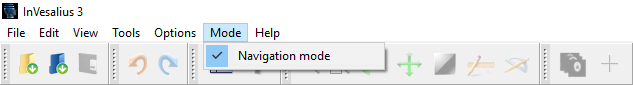
\includegraphics[scale=0.4]{nav_menu_en.png}
\caption{Menu to enable neuronavigation mode.}
\label{fig:nav_menu_en}
\end{figure}

\begin{figure}[!htb]
\centering
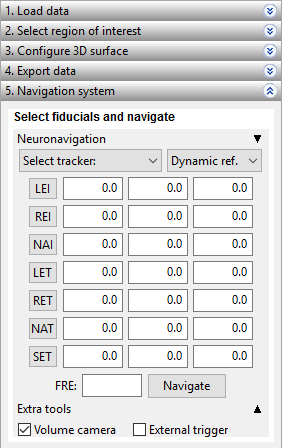
\includegraphics[scale=0.6]{nav_painel_en.png}
\caption{Tab for navigation system.}
\label{fig:nav_painel_en}
\end{figure}

\section{Spatial trackers and reference mode}

Currently, InVesalius Navigator supports three spatial tracking devices from two manufacturers, the MicronTracker
from ClaroNav (Toronto, Canada; figure~\ref{fig:tracker_claron}) and Fastrak, Isotrak and Patriot
from Polhemus (Colchester, United States; figure~\ref{fig:tracker_polhemus}).

After this, the first step is to choose the tracker in the menu \textbf{Select tracker:}, figure~\ref{fig:nav_select_tracker}.
The option \textbf{Debug tracker} allows the user to test the system even if none spatial tracker is connected.
This option simulates a spatial tracker by generating random coordinates.

\begin{figure}[!htb]
\centering
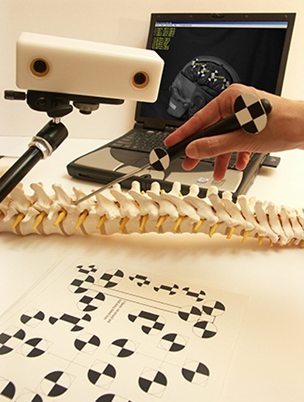
\includegraphics[scale=0.4]{tracker_claron.png}
\caption{ClaroNav MicronTracker - www.claronav.com/microntracker/.}
\label{fig:tracker_claron}
\end{figure}

\begin{figure}[!htb]
\centering
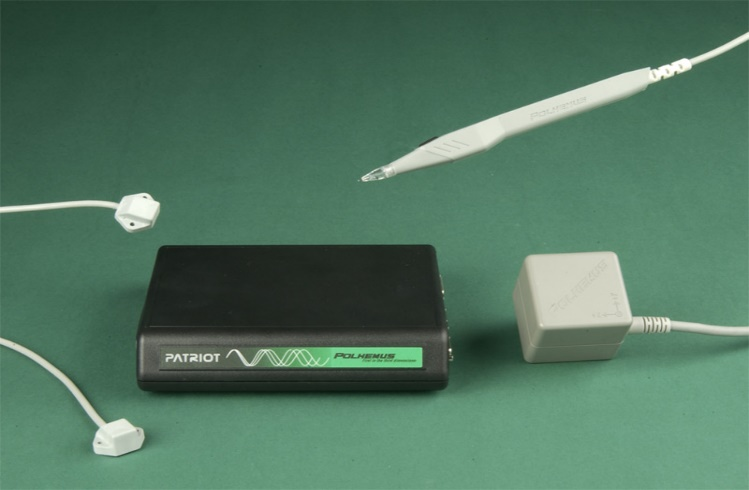
\includegraphics[scale=0.5]{tracker_polhemus.jpg}
\caption{Polhemus Patriot tracker - http://polhemus.com/motion-tracking/overview/.}
\label{fig:tracker_polhemus}
\end{figure}

\begin{figure}[!htb]
\centering
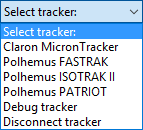
\includegraphics[scale=0.5]{nav_select_tracker_en.png}
\caption{Menu to select tracking device.}
\label{fig:nav_select_tracker}
\end{figure}

There are two references types to perform the navigation, static and dynamic (figure~\ref{fig:nav_menu_ref}).
Static mode uses just one spatial tracker probe. In this mode, the subject head must stay motionless after
registration (for more info about coregistration see section~\ref{sec:corregistro}). To avoid head movements artifacts,
a reference probe attached to some static part of the head is required, e.g. forehead. During neuronavigation
procedures, the reference probe will detect and correct the translation and rotation from the head.
This mode is known as dynamic reference.

\begin{figure}[!htb]
\centering
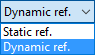
\includegraphics[scale=0.5]{nav_menu_ref_en.png}
\caption{Menu to select reference mode.}
\label{fig:nav_menu_ref}
\end{figure}

\section{Coregistration}
\label{sec:corregistro}

The aim of coregistration procedure is to find a relation that transforms a coordinate given in the tracking device space
to a coordinate in the virtual space (image). To perform the coregistration, the user must
use the function of \textbf{Correspondence between orientations axial, sagittal and coronal} (see section~\ref{sec:corresp_all_orient})
and select three anatomical fiducials in the image and then collect the same three fiducials with the spatial tracker.
The most common anatomical fiducials are the nasion and both tragus (ears). Figure~\ref{fig:nav_selec_coord} shows the fiducials panel.
When some image fiducial is selected, a marker (green sphere) is created in the volume, figure~\ref{fig:nav_balls_in_head}.

\begin{figure}[!htb]
\centering
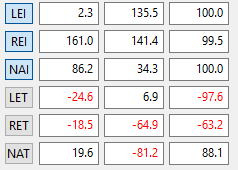
\includegraphics[scale=0.5]{nav_selec_coord_en.png}
\caption{Buttons and coordinates to select anatomical fiducials.}
\label{fig:nav_selec_coord}
\end{figure}

The buttons acronyms represent:

\begin{itemize}
	\item LEI: left ear in image
	\item REI: right ear in image
	\item NAI: nasion in image
	\item LET: left ear with spatial tracker
	\item RET: right ear with spatial tracker
	\item NAT: nasion with spatial tracker
\end{itemize}

\begin{figure}[!htb]
\centering
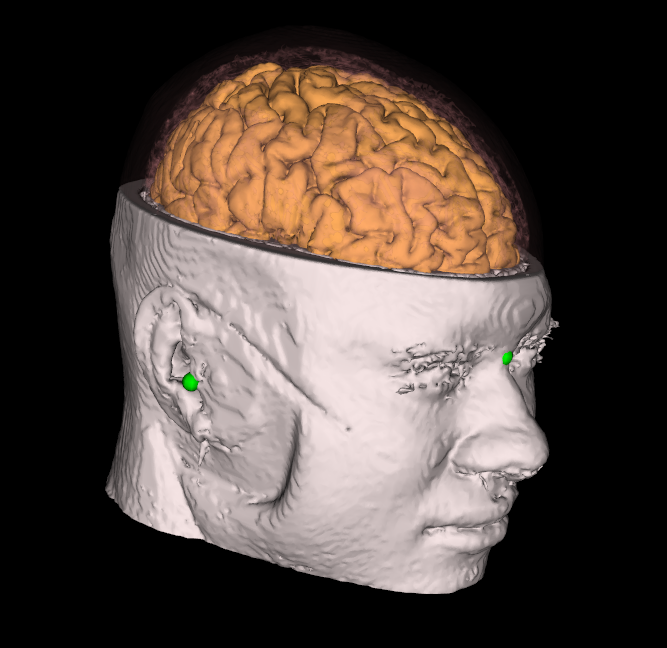
\includegraphics[scale=0.5]{nav_balls_in_head.png}
\caption{Selected fiducial markers represented as green spheres.}
\label{fig:nav_balls_in_head}
\end{figure}


\section{Fiducial registration error and navigation}

After all fiducials are selected in both spaces (tracker and image) the next step is to press button \textbf{Navegate}
button to start the neuronavigation. To stop navigation just press the button \textbf{Navigate} again.
Immediately after the navigation starts, the  \textit{Fiducial Registration Error} (FRE) is calculated. The FRE is the
root mean square distance between the image fiducials used for and after registration.

In the left side of navigate button there is a FRE text box. If FRE is high (greater than 3 mm) the navigation will not
be precise and the text box will become red, figure~\ref{fig:nav_fre_error}, it is recommended that the coregistration
is redone. Otherwise, if FRE is lower than 3 mm, the text box becomes green, showing that the navigation has an
acceptable precision, figure~\ref{fig:nav_fre_ok}.

\begin{figure}[!htb]
\centering
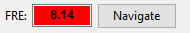
\includegraphics[scale=0.6]{nav_fre_error_en.png}
\caption{Navigation button and high FRE unsuitable for navigation.}
\label{fig:nav_fre_error}
\end{figure}

\begin{figure}[!htb]
\centering
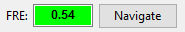
\includegraphics[scale=0.6]{nav_fre_ok_en.png}
\caption{Navigation button and low FRE suitable for navigation.}
\label{fig:nav_fre_ok}
\end{figure}

\section{Markers}

During navigation, it is possible to create sphere markers in the 3D volume. To do that, the user needs to select
\textbf{Extra tools} tab, figure~\ref{fig:nav_extra_tools}.

\begin{figure}[!htb]
\centering
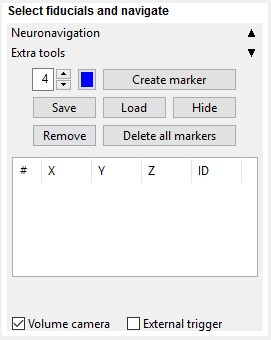
\includegraphics[scale=0.6]{nav_extra_tools_en.png}
\caption{Aba para manipulação de marcadores.}
\label{fig:nav_extra_tools}
\end{figure}

The marker creation will be positioned in the current red cross position. The size and color can be
changed, figure~\ref{fig:nav_vol_with_markers}.

When a marker is created, its coordinates appear in the list control. To identify one marker of the list control in the
volume, \textbf{double-click with left mouse button} the target item and the corresponding marker will blink.
To stop blinking the markers, the user just needs to select another marker, i.e. press once in another item.
It is also possible to create an ID to the marker, and to do that right click and select \textbf{Edit ID}, like
in figure ~\ref{fig:nav_id_list_markers}. Finally, a window will open allowing the user to create
the ID, figure~\ref{fig:nav_edit_id_markers}.

\begin{figure}[!htb]
\centering
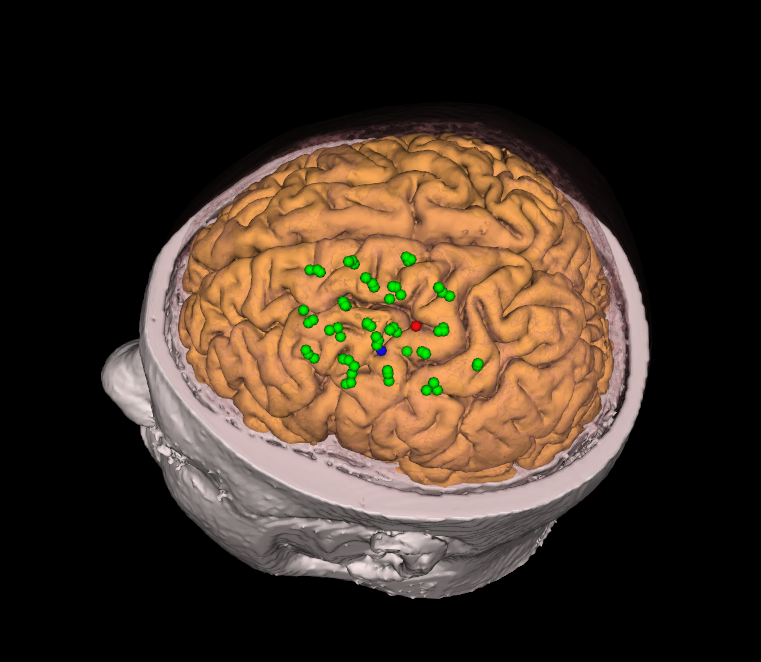
\includegraphics[scale=0.4]{nav_vol_with_markers.png}
\caption{Volume with different colors markers.}
\label{fig:nav_vol_with_markers}
\end{figure} 

\begin{figure}[!htb]
\centering
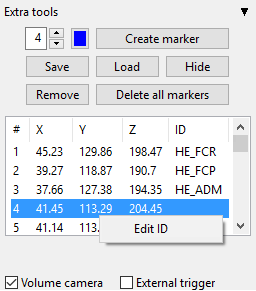
\includegraphics[scale=0.6]{nav_id_list_markers_en.png}
\caption{Task to manage marker creation.}
\label{fig:nav_id_list_markers}
\end{figure} 

\begin{figure}[!htb]
\centering
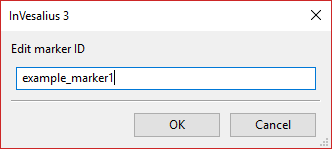
\includegraphics[scale=0.6]{nav_edit_id_markers_en.png}
\caption{Window to label the marker.}
\label{fig:nav_edit_id_markers}
\end{figure} 

The marker coordinates may be exported using the button \textbf{Save}. File extension is \textit{.mks}. This extension can be
opened in any word processor, e.g. Notepad or WordPad software. The file has the X, Y and Z coordinates followed by the RGB code,
marker size and ID. Posteriorly, the markers can be importated to the navigation system using button \textbf{Load}.

To remove markers, \textbf{select} one or as much markers needed to be deleted and press button \textbf{Remove}.
It is also possible to remove all markers, with the button \textbf{Remove all markers}. Another functionality
is to hide/show the markers in the volume using the \textbf{button show/hide}.


\section{External trigger checkbox}

Another way to create markers is using an external trigger. To activate this feature, just press the
checkbox \textbf{External trigger} before the navigation starts. This function was developed to communicate with
TMS devices, to create a marker whereas the pulses are applied. Besides, it is possible to adapt this function as
the user needs. The communication with the external device requires a serial port COM1. If this port receives
any RS-232 signal in 9600 \textit{baud rate} it will create a marker in the current red cross position.

\section{Camera volume checkbox}

The volume camera positioning is updated automatically, both by the red cross and the spatial tracker probe positioning.
The user can disable this function by unchecking the \textbf{Camera volume} checkbox.
Therefore, the camera has to be manually changed.
